
\section{Data Collection}
\label{sec:meth}

This section discusses how we collected and preprocessed data from VirusTotal.
We will present the analysis of these data in the next two sections.

\begin{table}[h!]
\centering
\footnotesize
{
%\begin{tabular}{@{\hspace{3pt}}l@{\hspace{3pt}}|@{\hspace{3pt}}c@{\hspace{3pt}}}
\begin{tabular}{l|l}
\hline
Metadata Fields & Explanation \\
\hline                            
%\cline{1-1}
{\bf name}      & file name of the submitted sample \\
{\bf timestamp} & timestamp for when the submission was made \\
{\bf source\_country} & the country from which the submission was made \\
{\bf source\_id} & user id of whom made the submission\\
{\bf tags} & providing more specific information for each {\bf type}\\
{\bf link} & where to download the submitted sample \\
{\bf size} & file size \\
{\bf type} & file type \\
{\bf first\_seen} & when the same sample was first submitted \\
{\bf last\_seen} & when the same sample was last submitted \\
{\bf hashes} & including sha1, sha256, vhash, md5, and ssdeep\\
{\bf total} & how many engines analyze the sample\\
{\bf positives} & how many engines identify the sample as malicious \\
{\bf positives\_delta} & changes in {\bf positives} fields \\
{\bf report} & detailed detection report from each AV engine \\
%\multicolumn{2}{|l|}
\hline

\end{tabular}
}
\mycaption{tab:fields}{VirusTotal Metadata.}
{ 
Fields for each submission retrieved from the VirusTotal private API and their relation explanation.
}
\end{table}





We downloaded the metadata and malware reports of all submitted files in November 2015 using the APIs VirusTotal provides,
resulting in a total of 43 million reports.
Table~\ref{tab:fields} shows the metadata fields and their meaning. 

\begin{figure}[t!]
\begin{center}
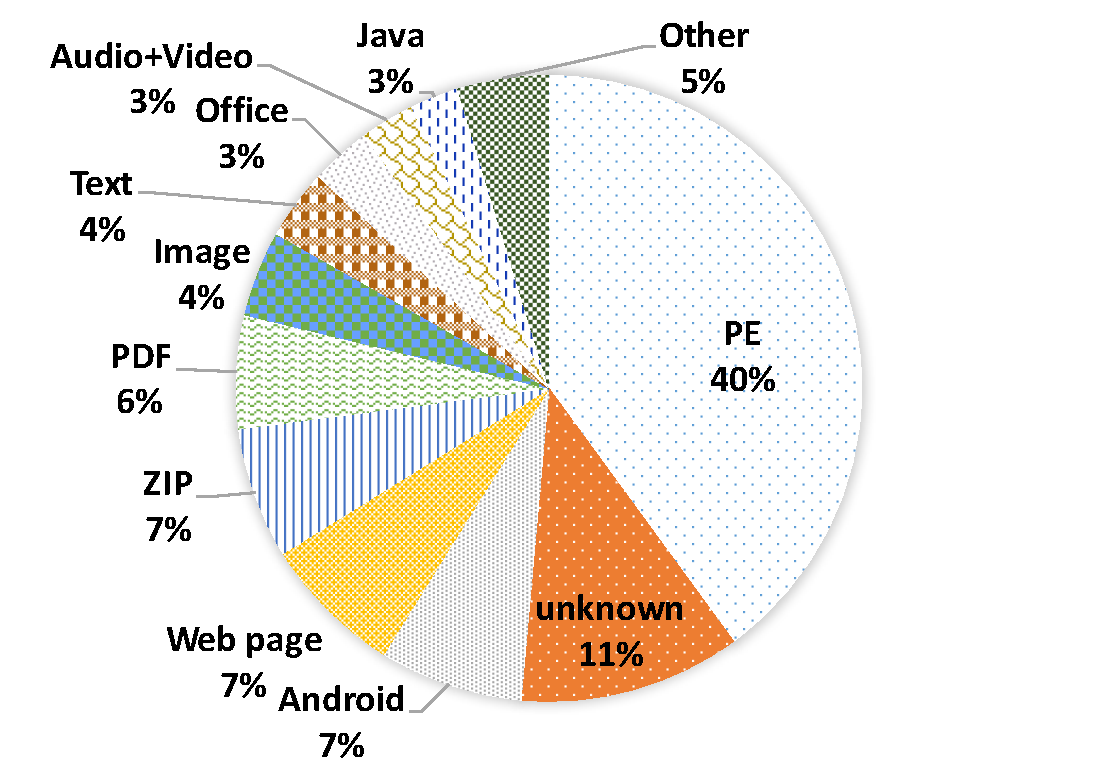
\includegraphics[width=2.5in]{figure/typePie}
\mycaption{fig:type}{File types for all submissions in November 2015.}
{File types and their distributions for all submissions on VirusTotal in November 2015.}
%\label{fig:new}
\end{center}
%\vspace{-0.3in}
\end{figure}


{\color{red} 
Figure~\ref{fig:type} shows file type distributions for all submissions. 
{\em Portable Executable (PE)}  files have the largest number of submissions. 
For around 11.5\% submissions, VirusTotal cannot figure out their file types. 
Malwares on Android have the third largest number of submissions.  
}

In this paper, we only focus on PE files 
and leave the analysis of other types of malicious files for future work. 
We filter all downloaded metadata by the type field. 
{\color{red} 
If the type field is either ``Win32EXE'' or ``Win32DLL'' tag, we consider the record as a PE file. 
Antivirus engines usually disagree with each other, so
we only rely on Microsoft antivirus engine to judge whether a PE file is a malware, because
Microsoft has a very good reputation in detecting PE malwares. 
}
Within the 43 million reports, 4.7 million are PE malwares. 
The number of reports, PE reports, and PE malwares submitted each day are shown in Figure~\ref{fig:subnum}.

The Microsoft antivirus engine classifies malwares into different names~\cite{microsoft}. 
We utilize this naming mechanism to decide what family a malware belong to.
Specifically, if two malwares have the same name under Microsoft engine, we consider them to be from the same family.

One caveat of VirusTotal is that it is possible that the VirusTotal APIs return redundant reports 
for the same submitted file. 
We use the combination of sha256 hash value and timestamp to detect and remove redundant reports.

After removing redundant reports, we find that most malwares were submitted only once to VirusTotal. 
Out of the total 4.7 million PE malware submissions, 4 million are distinct. 
On average, each PE malware was submitted 1.17 times to VirusTotal in November 2015. 
This observation is in contradictory to the common belief that most malwares are encountered by more than one user.
We suspect that the reason behind this low degree of repeated submissions by different users
is that VirusTotal users
tend to check whether their suspicious files have already been submitted recently
and avoid submitting redundant files.

%\textit{\underline{Threats to Validity.}}
Similar to all previous empirical studies, all our findings, experimental results, 
and conclusions need to be considered with our methodology in mind. 

The VirusTotal APIs only track which submission reports are sent to each downloader approximately, 
and there is no guarantee that all submission reports on VirusTotal can be downloaded successfully. 
Thus, it is possible that we missed some malwares submitted to VirusTotal. 
Also, we only leverage Microsoft antivirus engines to decide whether or not a submission is malicious, 
and it is possible that Microsoft antivirus engines cannot make this decision precisely. 
How to get a precise label for a PE file is out of the scope of this paper.  
Although there is a huge amount of malwares on VirusTotal, we believe that there are malwares never submitted to VirusTotal, 
and there are malwares submitted much later than when they appear in the real world.
Since there are no conceivable ways to study these malwares,
we believe that the malwares in our study provide a representative malware sample of the real world. 


